The corpus contains \WomenBooks{} works by \WomenAuthors{} women and
\MenBooks{} works by \MenAuthors{} men, which makes a comparison possible that
most eighteenth-century collections cannot support. We ask a narrow question
--- which concepts are used at noticeably different rates in the two sets ---
and take care to claim nothing wider than the answer allows.

The confounds come first, because they are large. The two sets differ in size
by a factor of five (\MenPassages{} passages against \WomenPassages{}). They
differ in date: the median dated passage by a woman is from
\WomenMedianYear{}, by a man from \MenMedianYear{}, a full generation apart.
And they differ in genre, because what survives and has been edited is not the
same for both: the women here are represented largely by devotional treatises,
letters and educational writing, the men substantially by natural-law
jurisprudence and academic moral philosophy. Any difference found below is a
difference between two \emph{collections}, produced by all three of those
factors at once. It is not evidence about authorship as such, and we do not
offer it as any.

\begin{figure}[t]
  \centering
  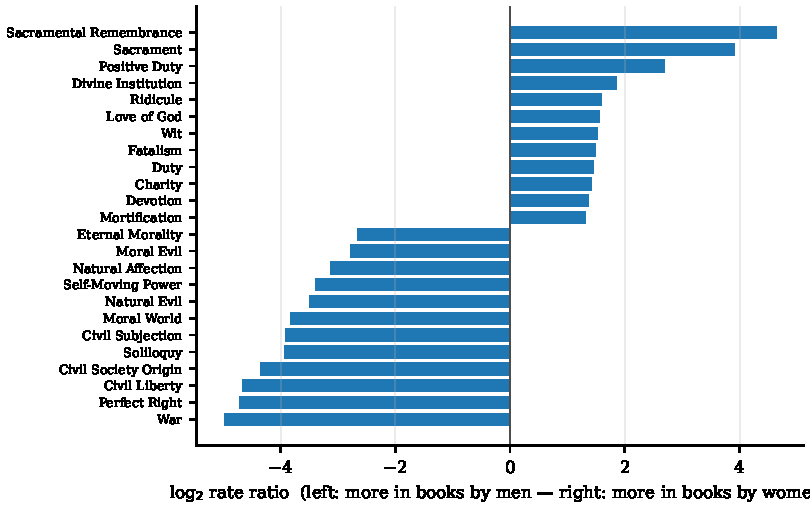
\includegraphics[width=0.92\linewidth]{authorship.pdf}
  \caption{Concepts with the most unequal rates between the two sets of books,
           as a log ratio. Only concepts appearing in at least five books on
           the leaning side are shown, so no single volume can produce an
           entry.}
  \label{fig:authorship}
\end{figure}

With that said, the separation is stark and clean. The concepts most
characteristic of the women's books are sacramental and devotional:
\concept{\TopWomenLean{}} leads at \TopWomenLeanRatio{} on a log$_2$ scale,
followed by \concept{Sacrament}, \concept{Positive Duty}, \concept{Divine
Institution} and \concept{Love of God}. The concepts most characteristic of
the men's books are political and juridical: \concept{\TopMenLean{}} at
$-\TopMenLeanRatio{}$, with \concept{Perfect Right}, \concept{Civil Liberty},
\concept{Civil Society Origin} and \concept{Civil Subjection} behind it.

Read carefully, this is a result about the shape of a discipline's archive
rather than about its authors. Moral philosophy in this period is written in
both registers --- the devotional and the juridical --- and the archive has
sorted them by the sex of the writer, because the institutional settings that
produced natural-law jurisprudence were closed to women and the devotional
tradition was not. The measurement recovers that sorting with considerable
precision. What it cannot do, and what no count of aliases could do, is
distinguish a writer choosing a register from a writer permitted only one.
